\documentclass[a4paper,11pt,oneside]{scrreprt}
\KOMAoptions{bookmarkpackage=false}

% ----------------------------------------------------------------------
% 字体配置：Palatino Linotype (西文) + 经典宋体/黑体/楷体搭配
% ----------------------------------------------------------------------
\usepackage{fontspec}
\setmainfont{Palatino Linotype}
\setsansfont{Arial}
\setmonofont{Consolas}[Scale=0.9]

\usepackage{xeCJK}
\setCJKmainfont{SimSun}[
    BoldFont={SimHei},
    ItalicFont={KaiTi}
]
\setCJKsansfont{SimHei}
\setCJKmonofont{SimSun}

% ----------------------------------------------------------------------
% 载入 ClassicThesis 样式宏包
% ----------------------------------------------------------------------
\usepackage[palatino=false,dottedtoc=true]{classicthesis}

% ----------------------------------------------------------------------
% 页面几何：置于 classicthesis 之后以生效舒适版面
% ----------------------------------------------------------------------
\usepackage{geometry}
\geometry{
    a4paper,
    left=2.6cm,
    right=2.6cm,
    top=3.0cm,
    bottom=3.2cm,
    headheight=18pt,
    headsep=24pt,
    footskip=30pt
}

% 基础工具宏包
\usepackage{booktabs}
\usepackage{graphicx}
\usepackage{tabularx}
\usepackage{array}
\usepackage{enumitem}
\usepackage{caption}
\usepackage{tcolorbox}
\tcbuselibrary{skins,breakable}

% ----------------------------------------------------------------------
% 目录超链接修复：确保直接点击标题文字即可跳转
% ----------------------------------------------------------------------
\renewcommand{\cftchapfont}{\normalfont\bfseries}
\renewcommand{\cftchappagefont}{\normalfont\color{CTMaroon}}
\renewcommand{\cftsecfont}{\normalfont}
\renewcommand{\cftsecpagefont}{\normalfont\color{CTMaroon}}
\renewcommand{\cftsubsecfont}{\normalfont\small}
\renewcommand{\cftsubsecpagefont}{\normalfont\small\color{CTMaroon}}

% 超链接设置（全局链接为红褐色，目录全文可点击跳转）
\definecolor{CTMaroon}{RGB}{128,0,0}
\definecolor{CTCharcoal}{RGB}{45,45,45}
\definecolor{CTWarmGray}{RGB}{249,248,245}
\definecolor{CTLightGray}{RGB}{242,242,242}

\hypersetup{
    unicode=true,
    colorlinks=true,
    linktoc=all,
    linktocpage=false,
    linkcolor=CTMaroon,
    citecolor=CTMaroon,
    urlcolor=CTMaroon,
    pdfstartview={FitH},
    pdfauthor={李鸿(2868014836@qq.com)},
    pdftitle={湖南大学 Robot 工作坊 2026 新生指南},
    pdfsubject={新生招新与技术进阶成长指南}
}

% 调优列表行距
\setlist{nosep,leftmargin=1.8em,topsep=4pt,partopsep=2pt,itemsep=3pt}

% 提示框设计
\newtcolorbox{ctbox}[1][]{
    enhanced,
    breakable,
    colback=CTWarmGray,
    colframe=CTMaroon,
    leftrule=2.5pt,
    rightrule=0pt,
    toprule=0pt,
    bottomrule=0pt,
    arc=0mm,
    boxsep=4pt,
    left=12pt,
    right=12pt,
    top=8pt,
    bottom=8pt,
    #1
}

% 行内代码微标
\newcommand{\inlinecode}[1]{%
    \colorbox{CTLightGray}{\texttt{\small #1}}%
}

% 图片与表格题注格式
\captionsetup{
    font={small,stretch=1.2},
    labelfont={color=CTMaroon,bf},
    labelsep=quad,
    justification=centering
}

\linespread{1.15} % 适度行距提升中文易读性

\begin{document}

% ======================================================================
% 扉页：ClassicThesis 风格标题页（带有工坊官方 Logo）
% ======================================================================
\begin{titlepage}
    \thispagestyle{empty}
    \begin{center}
        \vspace*{0.6cm}
        
        % 居中展示官方 Logo
        
\includegraphics[width=3.8cm]{assets/RobotWorkShop.jpg}\\[0.8cm]
        
        {\large\color{halfgray}\spacedallcaps{HUNAN UNIVERSITY $\cdot$ ROBOT WORKSHOP}}\\[0.3cm]
        {\footnotesize\color{halfgray}\spacedallcaps{Modern Engineering Training Center $\cdot$ 2026 Edition}}\\[1.5cm]
        
        {\fontsize{28}{34}\selectfont\color{CTMaroon}\textbf{湖南大学 Robot 工作坊}}\\[0.6cm]
        {\fontsize{20}{26}\selectfont\color{CTMaroon}\spacedlowsmallcaps{2026 级新生指南}}\\[1.4cm]
        
        \begin{quote}
            \centering\itshape\fontsize{10.5}{17}\selectfont\color{CTCharcoal}
            “学习的敌人是自己的满足，要认真学习一点东西，必须从不自满开始。\\
            对自己，‘学而不厌’，对人家，‘诲人不倦’，我们应取这种态度。”
        \end{quote}
        
        \vfill
        
        \begin{minipage}{0.85\textwidth}
            \centering\small\color{CTCharcoal}
            \rule{0.6\textwidth}{0.4pt}\\[0.5cm]
            \spacedlowsmallcaps{编著者：李鸿 (2868014836@qq.com)}\\[0.25cm]
            \textit{贡献者：江涛、李书淇、乔淼 等原著 $\cdot$ 历届队员与指导团队}\\[0.35cm]
            {\footnotesize\color{halfgray} 2026 年 9 月 $\cdot$ 长沙岳麓山下}
        \end{minipage}
        \vspace*{0.8cm}
    \end{center}
\end{titlepage}

% ======================================================================
% 前言部分（罗马数字页码）
% ======================================================================
\pagenumbering{roman}

\chapter*{前言：写在前面}
\phantomsection
\addcontentsline{toc}{chapter}{前言：写在前面}

各位 2026 级的新同学，欢迎了解并走进湖南大学现代工程训练中心 Robot 工作坊！

这份指南的最初版本由江涛、李书淇、乔淼等老学长结合工坊多年的摸爬滚打经验共同整理打磨而成。时光来到 2026 年，工坊的技术栈迎来了全面革新——具身智能（Embodied AI）与全自主双足人形机器人已成为我们的核心前沿业务；同时，传统的轮式格斗、智能清洁、四足机器狗等老牌赛事依然常青。

无论技术浪潮如何迭代，这份文档的初心从未改变仍然是 \textbf{带新成员一步步看清大学竞赛与工程学习的门道。}

\section*{答疑交流引路人}
\phantomsection
\addcontentsline{toc}{section}{答疑交流引路人}

大学期间遇到技术卡壳、学业迷茫、选课疑惑甚至生活问题，随时欢迎来工训中心与学长学姐面对面交流。你可以联系以下常驻工坊的学长学姐（信息持续更新中）：

\begin{center}
\small
\renewcommand{\arraystretch}{1.3}
\begin{tabularx}{\textwidth}{@{} l p{2.6cm} X @{}}
\toprule
\textbf{姓名 / 昵称} & \textbf{年级与专业} & \textbf{负责方向 / 专长标签} \\
\midrule
\textbf{刘辰宇} & 24电自 & 具身智能皇帝 \\
\textbf{李书淇} & 23智车 & 日常运维支柱，轮式格斗与 RoboCup 资深队员 \\
\textbf{马梓博} & 24自动化 & 嵌入式软件硬件 RoboCup人形组和电赛（备注：14号后集中答疑 命苦还债备考ing） \\
\textbf{张笑然} & 25电自 & 新生指导，主要赛项为轮式格斗，欢迎喜欢硬件方向的同学和我交流 \\
\textbf{曾维胜} & 24电子 & 志愿时长炼金术士 \\
\textbf{程佩娟} & 24通信 & RoboCup资深队员/人形 \\
\textbf{张雪雅} & 24电自 & 新媒体信号增强工程师 \\
\textbf{李鸿}   & 24电子 & RoboCup人形组，机器人运动会。AI4S \\
\textbf{胡杰佑} & 25智车 & 最懂sw之人，成图大赛最严厉的父亲 \\
\bottomrule
\end{tabularx}
\end{center}

同时，工坊能取得今天的成绩，离不开工训中心方璐、陈浩文老师的悉心指导与全方位资源支持；也离不开李路畅博士（信科院博士在读，工坊活化石）、任庸祥（电气院研究生在读，电自一哥、硬件神）、穆森源与申鑫洋（往届团长/副团长，技术元老与主力）等历届传奇前辈打下的坚实底座。

\clearpage

% ======================================================================
% 目录页（点击标题文字与页码皆可精准跳转）
% ======================================================================
\phantomsection
\pdfbookmark[0]{\contentsname}{tableofcontents}
\tableofcontents

\clearpage

% ======================================================================
% 第一章：工坊业务与竞赛全景
% ======================================================================
\pagenumbering{arabic}

\chapter{工坊业务与竞赛全景}

\section{核心领航赛事（具身智能重点业务）}

进入 2026 年，工坊全面发力具身智能（Embodied AI）与人形机器人技术。如:

\subsection{RoboCup 机器人世界杯（中国赛及国际赛·人形赛项）}

\begin{itemize}
    \item \textbf{赛事地位}：机器人领域全球顶流 A 类赛事。这是国内外含金量极高顶级对抗赛。目前全团队战略转向\textbf{【人形机器人足球赛项（Humanoid League）】}。
    \item \textbf{比赛本质}：让全自主双足人形机器人踏上真实绿茵场。比赛全程严禁任何遥控与场外人工干预，机器人需要仅依靠本体搭载的传感器（双目/单目相机、IMU、关节编码器），在剧烈碰撞、草皮摩擦和强光照变化下完成\textbf{感知、决策、双足行走、变向、射门与团队协作}。
    \item \textbf{四大核心研发小组与技能要求}：
\end{itemize}

\begin{figure}[htbp]
    \centering
    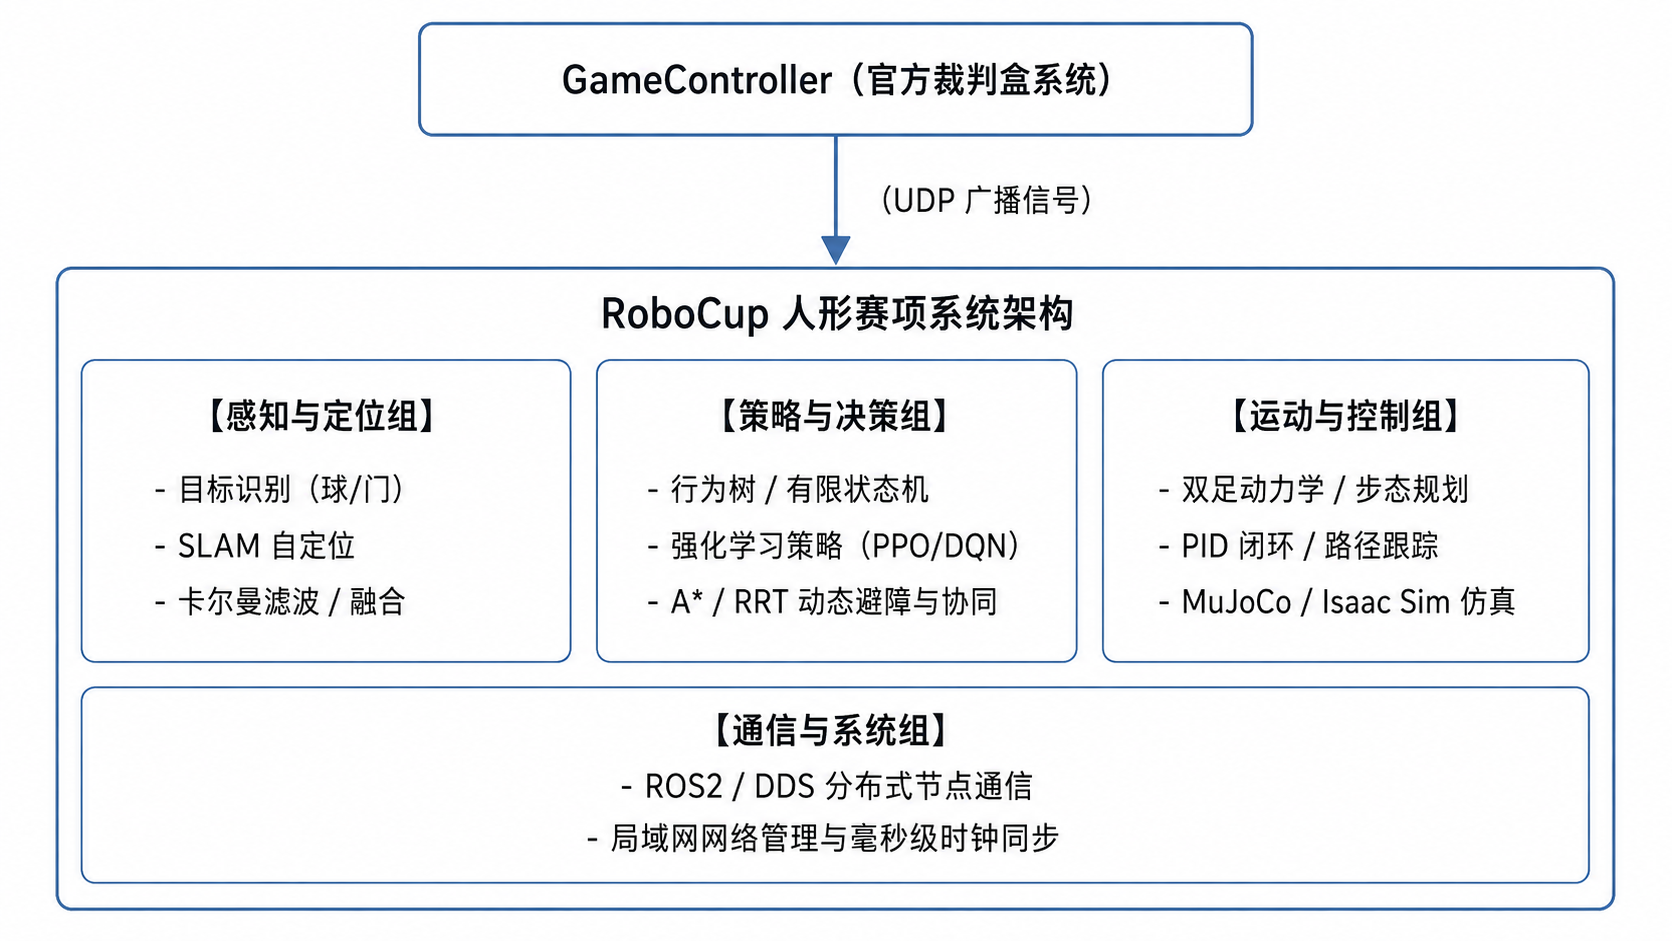
\includegraphics[width=0.88\textwidth]{assets/robocup_subgroups.png}
    \caption{RoboCup 人形机器人赛项四大核心研发小组架构}
\end{figure}

\begin{itemize}
    \item \textbf{感知与定位组}：主要负责图像处理与自身定位。利用摄像头、OpenCV、YOLO 等工具，在赛场上准确识别球、球门、队友与对手，并算清楚机器人在场地的实时位置坐标。
    \item \textbf{策略与决策组}：负责机器人的战术规划与动作调度。利用状态机、行为树或强化学习，自主决定机器人当前该带球突破、传球、远射还是防守，终极目标是打出默契的团队攻防配合。
    \item \textbf{运动与控制组}：负责双足机器人的平衡与步态控制。借助运动学规划与物理仿真平台（MuJoCo / Isaac Sim），训练机器人的各种踢球动作，以达到越过sim-to-real的gap。
    \item \textbf{通信与系统组}：负责多台机器人协同与裁判系统通信。解析官方 GameController 裁判盒发来的比赛信号（开球、暂停、比分），保障赛场局域网稳定通信。
\end{itemize}

\subsection{世界人形机器人运动会 （今年第一次参与）}

\begin{itemize}
    \item \textbf{赛事简介}：面对全球顶尖高校与创新科研机构的新一代人形机器人超级赛事。
    \item \textbf{竞赛特质}：工坊今年使用智元灵犀X2用于太极拳项目，主要涉及到的内容就是数据采集。惯性动捕，光学动捕，遥操使用，以及BVH文件的精修
\end{itemize}

\section{主力骨干赛事}

\begin{figure}[htbp]
    \centering
    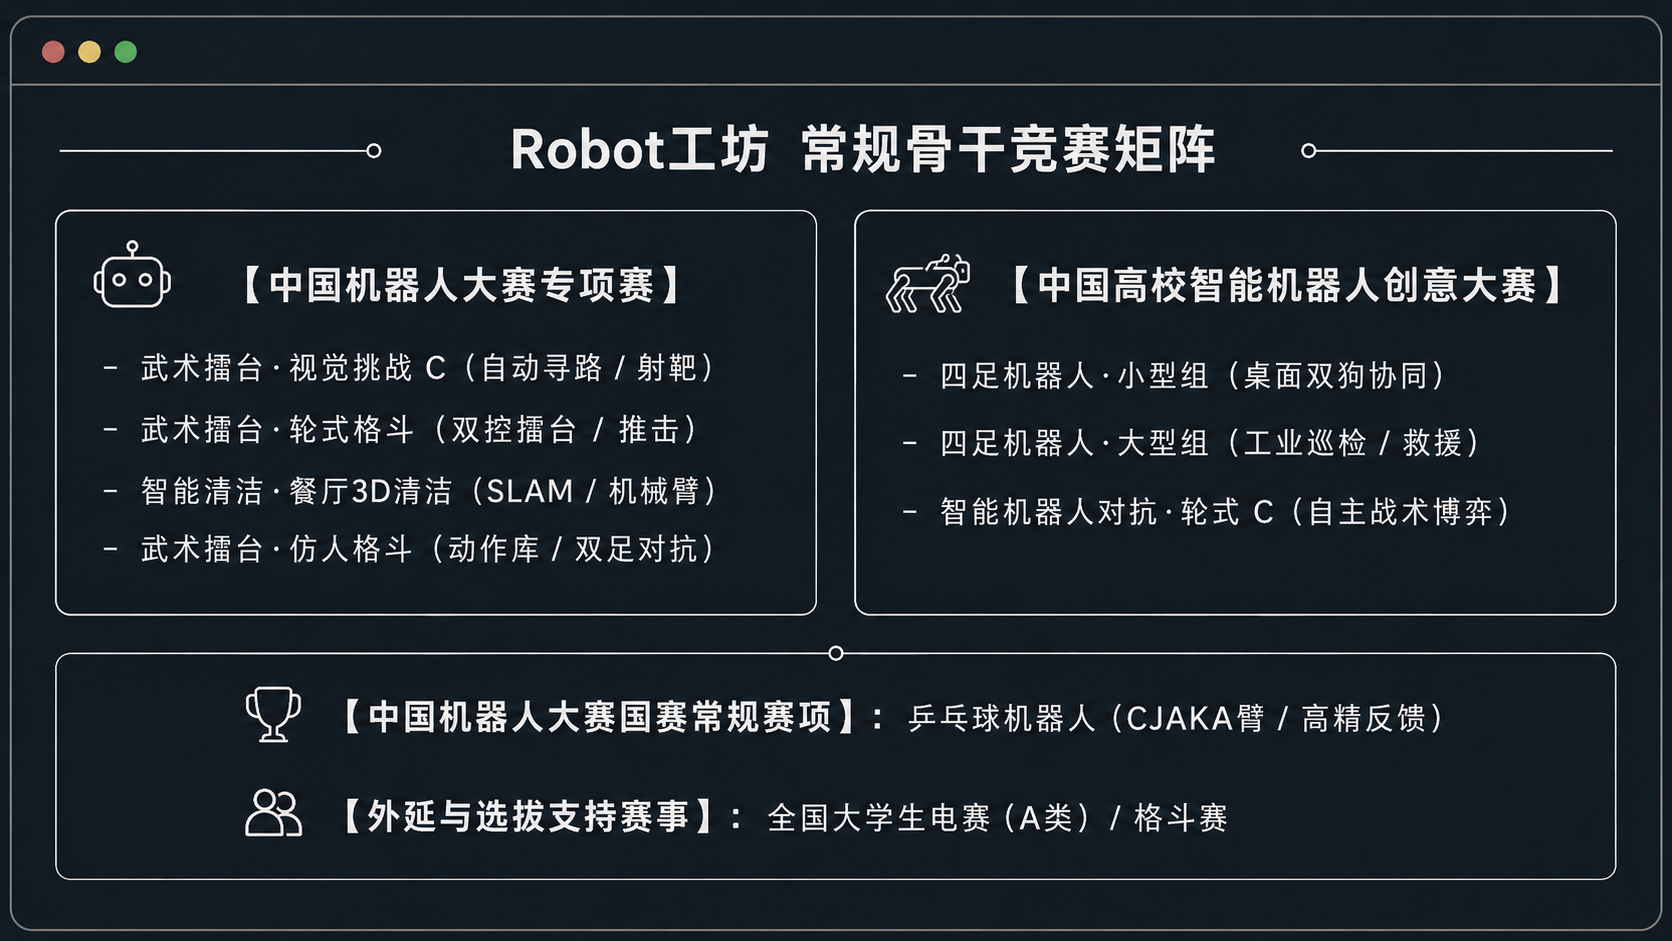
\includegraphics[width=0.92\textwidth]{assets/main_competitions.png}
    \caption{Robot工作坊主力赛事技术栈全景分布}
\end{figure}

本节介绍工坊常年参加的几个主力赛项。每年比赛规则都会微调，但所需技能基本大同小异，供大家参考定位。技能会在第二章详细介绍。

\subsection{中国机器人大赛专项赛（一般每年8月）}

中国机器人大赛专项赛相当于国赛的预选赛。参赛队伍较多的赛项需要先在专项赛选拔，\textbf{只要专项赛晋级，国赛大概率有保底三等奖}，获奖比例也相对更高（一等奖约20\%、二等奖约30\%、三等奖约40\%）。

\begin{itemize}
    \item \textbf{(1) 武术擂台赛 - 视觉挑战}
    \begin{itemize}
        \item \textbf{简介}：给小车一张地图，让机器人在场地内根据路径点自动寻路、避障，最后用车载激光模块射倒指定标靶。全自主运行，不需要现场手动操作，比较考验软件应用能力。
        \item \textbf{所需技能}：Python / C++、Linux终端、ROS基础与导航、视觉OpenCV。
    \end{itemize}
    \item \textbf{(2) 武术擂台赛 - 轮式自主格斗}
    \begin{itemize}
        \item \textbf{简介}：工坊老牌王牌项目。两台机器人在擂台上全自主对抗，要能自动识别台面边缘防跌落，还要识别对手把它推下去，同时抢夺场上的能量块加分。软硬件高度结合，工作量较大，涉及知识面较广。
        \item \textbf{所需技能}：C/C++、Python、嵌入式（单片机）、SolidWorks机械建模、嘉立创EDA画板、视觉OpenCV。
    \end{itemize}
    \item \textbf{(3) 智能清洁机器人 - 餐厅3D清洁}
    \begin{itemize}
        \item \textbf{简介}：轮式底盘加装 5 自由度机械臂，在模拟餐厅里自主建图导航、识别餐盘和垃圾、抓取并分类扔进垃圾箱。软硬件结合紧密，考验机械臂和底盘协同。
        \item \textbf{所需技能}：C++ / Python、Linux (Ubuntu)、ROS、激光/视觉SLAM导航、视觉OpenCV、机械臂逆解。
    \end{itemize}
    \item \textbf{(4) 武术擂台赛 - 仿人格斗}
    \begin{itemize}
        \item \textbf{简介}：小型双足人形机器人擂台格斗对抗，主要靠舵机控制和动作库编写。
        \item \textbf{所需技能}：C语言、嵌入式开发、舵机控制、姿态平衡。
    \end{itemize}
\end{itemize}

\subsection{中国高校智能机器人创意大赛（简称创意赛，6月预选，8月国赛）}

学校非常重视的高水平比赛，技术难度与含金量都很高。

\begin{itemize}
    \item \textbf{(1) 四足机器人（小型组）}
    \begin{itemize}
        \item \textbf{简介}：模拟两台桌面级小型四足机器狗协同作业，危险标志识别、避障并一起搬运物品。
        \item \textbf{所需技能}：Python / C++、Linux、视觉OpenCV、基础步态控制、SolidWorks。
    \end{itemize}
    \item \textbf{(2) 四足机器人（大型组）}
    \begin{itemize}
        \item \textbf{简介}：工业级大机器狗，模拟工业巡检场景，完成复杂地形越障、巡检、救援与抓取任务。代表了更高的技术门槛。
        \item \textbf{所需技能}：ROS、Nav导航、Python / C++、Linux、视觉OpenCV、SLAM。
    \end{itemize}
    \item \textbf{(3) 智能机器人对抗赛（轮式对抗）}
    \begin{itemize}
        \item \textbf{简介}：双车自主攻防对抗，包含雷达测距走位与自瞄博弈，考验自主算法与抗干扰能力。
        \item \textbf{所需技能}：C/C++、嵌入式、ROS、视觉。
    \end{itemize}
\end{itemize}

\setcounter{subsection}{3}
\subsection{拓展介绍：电赛}

\begin{itemize}
    \item \textbf{电赛（全国大学生电子设计竞赛，A类）}：非工坊主力参赛序列，由工训中心统一组织，3人一组封闭比赛 4 天 3 夜。含金量极高，想打电赛必须精通嵌入式和模电数电，工坊有充足的示波器和实验设备支持大家备赛。
\end{itemize}

\clearpage

% ----------------------------------------------------------------------
% 1.3 训练营及校企表格排版
% ----------------------------------------------------------------------
\section{训练营}

工作坊始终坚持“前沿探索、创新实践、产教融合”的育人理念。除了每年常规的机器人赛事，工坊深度依托湖南大学现代工程训练中心，与阿里巴巴达摩院、Datawhale、中联重科旗下中科云谷、火山引擎等头部科研机构与大厂联合打造高水平实训营：

\subsection{校企产教融合实训（校企训练营并不固定，以下是往期训练营展示）}

\begin{center}
\small
\renewcommand{\arraystretch}{1.35}
\setlength{\tabcolsep}{4pt}
\begin{tabularx}{\textwidth}{@{} c >{\raggedright\arraybackslash}p{3.0cm} >{\raggedright\arraybackslash}X >{\raggedright\arraybackslash}p{2.6cm} c c @{}}
\toprule
\textbf{年度} & \textbf{训练营名称} & \textbf{项目简介与核心内容} & \textbf{合作企业 / 机构} & \textbf{人数} & \textbf{推文回顾} \\
\midrule
\textbf{2025} & 乐云具身·SparkEdu 湖南大学站 & 开源机械臂实操，具身 VLA 模型体验与部署，涵盖从数据遥操作采集到模型微调、再到物理本体部署的全链路。 & 达摩院 DAMO 开发者矩阵、Datawhale & 60 人 & \href{https://mp.weixin.qq.com/s/ihzD-yhNVHQPK1FejKWDNQ}{\underline{回顾推文}} \\
\midrule
\textbf{2026} & 具身智能创新实践训练营 & 以“前沿探索，实战赋能”为主题，聚焦全尺寸双足人形机器人开发全链路能力与实机控制。 & 中科云谷（中联重科旗下） & 31 人 & \href{https://mp.weixin.qq.com/s/E1cUX-PR-QRzz49iwjcRkg}{\underline{结营报道}} \\
\midrule
\textbf{2026} & AI+X高校行·百校用虾大会 湖南大学站 & 全国首站。围绕 OpenClaw 智能体展开：一阶“养虾/用虾”环境搭建与部署；二阶线上真实业务智能体任务开发与百校评审。 & Datawhale、火山引擎 & 138 人 & \href{https://mp.weixin.qq.com/s/jr7Jtku0GMDiRccZIJmcdg}{\underline{现场盛况}} \\
\midrule
\textbf{2026} & 抖音创变者计划黑客松联赛 & 长沙城市交流赛（覆盖长沙各大高校）。围绕 AI 创新产品搭建创意狂欢舞台，让“小而美”的 AI 创意加速孵化落地。 & 抖音 AI 创变者计划 & 110 人 & \href{https://mp.weixin.qq.com/s/maKGxujJ5bABPwvlARMFmg}{\underline{相关链接}} \\
\bottomrule
\end{tabularx}
\captionof{table}{往期校企联合实训营展示}
\end{center}

\vspace{0.5cm}

\subsection{工坊寒假精英训练营（成为正式主力队员的必经之路）}

\begin{itemize}
    \item \textbf{训练营定位}：工坊每年最核心的人才孵化项目，专为有志于在次年征战 RoboCup 人形赛、中国机器人大赛及创意赛的新生打造。
    \item \textbf{时间节奏}：每年寒假期间（通常为 1 月中旬至 2 月中旬，为期整 4 周）。
    \item \textbf{运行机制}：
    \begin{enumerate}
        \item \textbf{周计划追踪}：入营同学每周需拟定一份量化学习计划，周末提交代码、学习笔记或实物视频成果，由各方向学长负责人严格审阅并打分，打分直接计入年终遴选总成绩。
        \item \textbf{双轨制闭环考核}：
        \begin{itemize}
            \item \textbf{统一基础考核}：基础软件方向（C语言编程机考与算法补全）或基础硬件方向（立创 EDA 原理图与 PCB 走线设计 / SolidWorks 机械建模二选一）。
            \item \textbf{进阶技术栈答辩考核}：涵盖 Linux/Ubuntu、ROS/ROS2、计算机视觉（OpenCV）、具身智能与强化学习等。开学第一周进行线下 PPT 答辩与实机现场演示，由资深学长及指导老师面对面技术质询。
        \end{itemize}
    \end{enumerate}
\end{itemize}

% ======================================================================
% 第二章：技能树与学长秘籍
% ======================================================================
\chapter{技能树与学长秘籍}

很多大一新生刚入校时都会被“嵌入式、SLAM、深度学习、运动学”等一连串高大上的名词吓退。需要明确的是：\textbf{童子功不是进工坊的必须要求，工坊的绝大多数国一选手大一开学时也连代码都没写过！} 关键在于\textbf{合理的学习路线，以及懂得借力现代 AI 辅助学习}。

\section{基础技能（大一入门必修）}

基础技能其实最吃基本功。基础不牢，地动山摇。我们目前的硬性考核要求是：\textbf{所有大一新生必须先学扎实 C 语言}。

\subsection{软件基础}

\subsubsection*{(1) C 语言（核心基石·11月小考核唯一科目）}

C 语言是高级语言里的底层语言。工科专业做机器人，底层的单片机（STM32、Luby、51）、树莓派外设驱动、电机的 PWM 调速、通信协议解析全是 C/C++。学好了 C 语言，你对内存、指针、堆栈和程序运行逻辑会有最真实的触觉，再转去学 Python 或 C++ 就像看白话文一样顺畅。

\begin{itemize}
    \item \textbf{学到什么程度就够考核了？}
    秋季阶段（10-11月），\textbf{大家只需学到“指针前一章”即可！} 指针难度较大，大一初期不着急深入；重点是吃透：\textbf{基本变量类型、运算符与表达式、条件分支（if-else/switch）、循环结构（for/while）、数组与函数调用}。这些将是 11 月下旬闭卷小考核的核心范围。学有余力的同学，建议提前看一看 \textbf{C++ 的“类（Class）”与面向对象概念}，这在后续 ROS 节点开发中经常用到。
    \item \textbf{精品网课推荐（二选一即可，重在亲手敲代码）：}
    \begin{enumerate}
        \item \textbf{浙江大学·翁恺老师《C语言程序设计》}：\href{https://www.bilibili.com/video/BV1dr4y1n7vA/}{\underline{B站链接}}
        \begin{itemize}
            \item \textit{特点}：大师级讲授，娓娓道来，重在计算机底层逻辑与概念本质，极度适合零基础小白建立扎实的编程认知。
        \end{itemize}
        \item \textbf{黑马程序员《C语言零基础入门到精通》}：\href{https://www.bilibili.com/video/BV1Xa4y1k7LU/}{\underline{B站链接}}
        \begin{itemize}
            \item \textit{特点}：偏向工程实战与速成，配套随堂练习与小案例丰富，适合喜欢通过刷题敲代码快速掌握语法的同学。
        \end{itemize}
    \end{enumerate}
\end{itemize}

\subsubsection*{(2) Python}

Python语法极其简洁，不需要繁琐的环境底层配置，各种现成库（OpenCV、NumPy、PyTorch、ROS rclpy）极其健全。随着AI 的爆发，Python的使用范围也在扩大。
学完C语言后，Python基本手到擒来，这里就不推荐网课了，想看的话网上资源也很多。

\subsubsection*{(3) Java}

\begin{itemize}
    \item Robot工坊目前的全部比赛和研发，完全用不到 Java！
    \item Java 主要用于互联网企业级后端、安卓原生开发或大数据分布式系统开发。如果你是软件工程/计算机专业的同学，未来目标非常明确地想去互联网大厂做后端开发，科班课程自会教授；如果你的目标是机器人与嵌入式软硬件，大一大二不必在 Java 上花费宝贵的时间。
\end{itemize}

\subsection{硬件基础}

硬件开发主要由“机械结构”与“电路 PCB”两大支柱构成。现代工具的使用门槛已经大幅降低，小白跟着教程练习三五天都能画出像模像样的零件和板子；难点在于背后的\textbf{工程常识与实战经验}。

\subsubsection*{(1) SolidWorks（3D 机械结构建模与打样）}

\begin{itemize}
    \item \textbf{应用场景}：工坊拥有数台高精度 3D 打印机。轮式格斗车的防掀铲斗、激光雷达云台、深度相机避震外壳、四足狗腿部连杆与法兰盘，全由队员在 SolidWorks 里建模并 3D 打印加工。
    \item \textbf{学长建议}：学会“草图绘制、拉伸凸台、切除、圆角、倒角、装配体与工程图”等核心操作只需 3 天。画结构时要多考虑物理现实：螺丝沉头预留多大孔径？3D 打印耗材（PLA/PETG/ABS）的收缩率公差要留多少？薄壁受力会不会脆断？这些多去工坊找学长摸摸零件就会懂。
    \item \textbf{精品网课推荐}：
    \begin{itemize}
        \item 【SolidWorks七天速成教程】2025最新最全快速精通教程：\href{https://www.bilibili.com/video/BV1Qr32zcEFy/}{\underline{B站链接}}
    \end{itemize}
\end{itemize}

\subsubsection*{(2) 立创 EDA}

\begin{itemize}
    \item \textbf{为什么推荐立创 EDA 而非老牌 Altium Designer (AD)？}
    对于入门而言，AD 安装包十几 GB、需要破解且没有云端封装库，极其劝退新手；而\textbf{立创 EDA（专业版）}支持国产网页端/客户端免配置直接运行，无缝直连嘉立创商城数百万级元器件库（自带 3D 模型与封装），画好原理图一键转 PCB 走线，还能直接导出生产文件送厂免费打样（学生每个月可领免费打样券！）。
    \item \textbf{实战应用}：做机器人往往空间极其狭小，市面买来的降压模块和驱动板尺寸不合适，必须自行画板，将单片机最小系统、电源稳压（12V转5V/3.3V）、MOS管电机驱动与排针接口整合在一张板子上。
    \item \textbf{精品网课推荐}：
    \begin{itemize}
        \item 【国一学长带你学嘉立创EDA专业版 全程保姆级教学】：\href{https://www.bilibili.com/video/BV1At421h7Ui/}{\underline{B站链接}}
    \end{itemize}
\end{itemize}

\section{进阶技术栈（选学与答辩方向）}

\begin{ctbox}
\textbf{提示}：进阶技术栈是基于你有良好编程基础与工科兴趣之上的拓展。大一上学期切忌贪多求全，先稳扎稳打夯实 C 语言，寒假再根据队伍与兴趣挑 1-2 门主攻！
\end{ctbox}

\subsection{嵌入式开发}

基本很多公司都需要嵌入式开发岗，岗位职责是用极低的成本完成目标功能。入门的话，可以从51单片机或者32单片机入手，如果精力充足，建议可以先学51,再学32。因为51单片机没有库函数，所有编程开发都是基于硬件底层，所以学习的过程中更能理解底层硬件电路的设计逻辑，懂得底层后才好去上手新的芯片，这就需要自己去查阅数据手册，所以最开始学习起来可能会比较吃力。32单片机是有库函数的（最主流的是标准库和HAL库，但标准库似乎没有再继续维护了,会一种库函数就行，另一种就能看懂），有库函数就会简单许多，不用管底层，调函数来用就行。

\begin{itemize}
    \item \textbf{神级网课推荐（全网公认必看）}：
    \begin{itemize}
        \item \textbf{江协科技《STM32入门教程》}：\href{https://www.bilibili.com/video/BV1th411z7sn/}{\underline{B站链接}} —— \textit{被无数工科生奉为神作的 STM32 教学，讲解深入浅出，代码逐行手打，看这一个就够了！}
        \item \textbf{铁头山羊《STM32入门教程新版》}：\href{https://www.bilibili.com/video/BV11X4y1j7si/}{\underline{B站链接}} —— \textit{注重工程化与代码规范，非常适合进阶参考。}
    \end{itemize}
\end{itemize}

\subsection{Linux / Ubuntu}

Linux是一个操作系统，相比于嵌入式，它的开发就简单许多（但成本也会更高，毕竟一般的嵌入式板子没有足够的内存来安装操作系统），可以脱离底层，相当于它已经帮你完美地把硬件底层和软件开发联系起来，所以你不需要知道底层硬件的运行逻辑（如处理器如何多线程运算，通信如何实现等），你只需要在终端敲Linux指令就能实现开发（如调用USB设备等都是一条指令的事），所以你得熟悉Linux指令集。
Linux就是一些指令，没啥网课，多敲敲指令就行。

\begin{itemize}
    \item \textbf{新手安装指南}：建议大一新生在自己电脑上通过 \textbf{VMware Workstation} 虚拟机安装 \textbf{Ubuntu 20.04 或 22.04 LTS}（有能力的同学可安装 Windows + Ubuntu 双系统）。学会换国内清华/阿里镜像源、安装中文输入法、掌握 \texttt{cd}, \texttt{ls}, \texttt{sudo}, \texttt{chmod}, \texttt{cp}, \texttt{mv}, \texttt{rm}, \texttt{ping}, \texttt{ifconfig} 等常用指令，复杂配置直接借助 AI 指引。
\end{itemize}

\subsection{ROS2}

ROS可以理解为针对机器人开发的一种Linux的子系统，安装在ubuntu系统（ubuntu系统是Linux的一个发行版）上，ROS的使用极为广泛，基本有机器人的地方就有ROS，路径规划、自主导航、图像处理、机械臂控制等等都可以用ROS来开发，但你想学习ROS的话，前提得知道Linux指令（可以不用刻意去专门学习，经常用的指令就那么几条，用得多了自然就会了）。

\begin{itemize}
    \item \textbf{必备利器与网课推荐}：
    \begin{itemize}
        \item \textbf{鱼香ROS一键安装}：终端运行一行指令即可一键搞定 Ubuntu 换源、ROS2 快速安装与环境依赖：\\
        \inlinecode{wget http://fishros.com/install -O fishros \&\& . fishros}
        \item \textbf{古月居《古月·ROS2入门21讲》}：\href{https://www.bilibili.com/video/BV1gr4y1Q7j5/}{\underline{B站链接}} —— \textit{概念清晰，新手必看。}
    \end{itemize}
\end{itemize}

\subsection{CV（计算机视觉）}

CV可以理解为程序开发中专门针对图像的一个研究方向，也是AI领域很热门的方向,但是比赛中只会涉及部分简单的应用，比如颜色识别，人脸识别，二维码识别，特征匹配等，在robocup中还涉及图像畸变等更进阶的内容。
CV是一个很大的方向，最常用最便捷的是python中的openCV库，不用太专门去学，看看就好，要用的时候可以直接AI。

\begin{itemize}
    \item \textbf{推荐网课}：
    \begin{itemize}
        \item 【黑马程序员 10小时学会OpenCV入门教程】：\href{https://www.bilibili.com/video/BV1Fo4y1d7JL/}{\underline{B站链接}}
    \end{itemize}
\end{itemize}

\subsection{AI 与具身智能}

进入 2026 年，大模型与具身智能极大拓宽了大学生的实践边界。工坊与全国顶尖 AI 开源社区 \textbf{Datawhale} 深度合作，推荐大家沿以下开源体系进阶：

\begin{itemize}
    \item \textbf{Datawhale 开源精品学习地图}：
    \begin{itemize}
        \item \textbf{智能体实战}：\href{https://github.com/datawhalechina/hello-agents}{\underline{Hello-Agents 智能体教程}} —— 从 0 到 1 打造自主决策 Agent；
        \item \textbf{大模型应用}：\href{https://github.com/datawhalechina/happy-llm}{\underline{Happy-LLM 快乐学大语言模型}} —— 掌握 Prompt Engineering、微调与 API 调用；
        \item \textbf{现代开发范式}：\href{https://github.com/datawhalechina/easy-vibe}{\underline{Easy-Vibe (Vibe Coding 指南)}} —— 学习如何与 AI 结对编程；
        \item \textbf{知识检索}：\href{https://github.com/datawhalechina/all-in-rag}{\underline{All-in-RAG 全栈指南}} —— 构建工坊与团队专属知识库；
        \item \textbf{强化学习基础}：\href{https://github.com/datawhalechina/easy-rl}{\underline{蘑菇书 Easy-RL}} —— 结合 OpenAI Gym / Gymnasium 学习 PPO、DQN 算法，专为人形策略与四足步态打底。
    \end{itemize}
    \item \textbf{前沿具身平台与物理动力学仿真}：
    \begin{itemize}
        \item \textbf{VLA（Vision-Language-Action）大模型实操}：将自然语言指令与视觉输入直接映射为机械臂与机器人的末端控制动作；
        \item \textbf{物理仿真环境}：
        \begin{itemize}
            \item \textbf{MuJoCo}：极速、精确的多体接触动力学仿真，适合四足与双足步态快速收敛；
            \item \textbf{NVIDIA Isaac Sim / Isaac Lab}：\href{https://www.bilibili.com/video/BV1X1RZYfE7Z/}{\underline{B站配置与入门指南}}，依托 GPU 并行仿真几千台机器人进行强化学习超快加速训练，是未来具身算法上实机前的黄金测试床。
        \end{itemize}
    \end{itemize}
\end{itemize}

% ======================================================================
% 第三章：学习安排与考核选拔
% ======================================================================
\chapter{学习安排与考核选拔}

考虑到各位的编程基础以及编程的重要性，所以我们的大致安排是各位\textbf{先学习 C 语言}，学习时间大约为一个月左右，之后我们会有一个简单的考核，考核通过后方可加入工坊。

\begin{ctbox}
\textbf{注意}：今后工坊的管理层成员换届以及参赛队员的选拔都会从这次考核通过的人中选，然后各位就可以按照个人意愿选择学习软硬件以及进阶技术，寒假后会再次进行考核以选拔参赛队员。
\end{ctbox}

\section*{10月-11月（小考核）：}
\phantomsection
\addcontentsline{toc}{section}{10月-11月（小考核）：}

先打好编程基础，花一个月左右时间去学习 C 语言，至少学到指针前一章（黑马程序员的网课，翁恺的网课也差不多，指针可以不着急学，指针挺难的，而且比赛不怎么用，然后就是需要去学习一下 C++ 的类，比赛中有的地方会用到）。

\begin{itemize}
    \item \textbf{考核范围}：C 语言，不包括指针
    \item \textbf{考核题型}：暂定为程序补全、程序阅读、语法判断等基础题目
    \item \textbf{考核形式}：11 月份下旬（具体时间待定，我们会避开期中考试）我们会进行考核，考核内容不难，就一些基本的语法。考核形式为\textbf{闭卷线下考试}，携带个人电脑到指定考场考试，\textbf{不允许上网以及使用 AI}（基本语法都要上网查的话也是没救了，而且 IDE 是会有智能补全和提示的），只能使用自己的编译器来写代码，自行调试后把代码提交到指定网址。一经发现有作弊行为，之后将与工坊再无交集。
    \item \textbf{定位}：小考核并不是为了选拔队员而存在，而是为了筛选有自主解决问题和基本编程能力的同学，也就是有一定学习能力的同学，但难度不会太难，通过率预计很高。
\end{itemize}

\section*{12月-下学期开学（大考核）：}
\phantomsection
\addcontentsline{toc}{section}{12月-下学期开学（大考核）：}

重点是在寒假自学，但也不希望占用太多时间，毕竟第一个假期嘛。这个学期的后半段可以先好好准备期末考试，寒假之前我们会再出一个学习以及考核的文档。

\begin{itemize}
    \item 第一次考核通过后，各位就可以根据自己的兴趣自行去学习。寒假的时候会安排寒假训练营，以比赛为主线学一些具体技术（具体安排到时候会出），下学期开学后安排考核。
    \item \textbf{基础技能考核}：分软件和硬件两个方向（有能力的完全可以俩都学，技多不压身），考核方式待定。
    \item \textbf{进阶技术栈考核}：（如果觉得自己能力有限，可以先不学进阶技术栈的东西，先把基础打好，基础不牢地动山摇）采用线下考查的方式，即带上任何你觉得能反映你学习成果的东西来当面问答。
\end{itemize}

\section*{下学期开学后：}
\phantomsection
\addcontentsline{toc}{section}{下学期开学后：}

我们会根据前面的考核结果挑选参赛队员，以及管理层的换届成员（管理层包括综合部、技术部、宣传部等，主要负责工坊的日常管理、宣传招新、赛事信息、志愿时长等，到时候会提交简历进行面试选拔）。

\begin{itemize}
    \item 管理层成员因为劳动会比纯打比赛的同学多一些，因而会被重点培养与考察，比赛排位也会推荐靠前，以及接触更多比赛之外的工坊各大项目等丰富简历的机会。
    \item 打比赛需要技术，但技术不应该为唯一评判准则，更不应以一个个量化的符号生硬地选拔同学，应该重视综合素质，重视每个同学的发展需求。
\end{itemize}

% ======================================================================
% 第四章：软件及网站推荐
% ======================================================================
\chapter{软件及网站推荐}
\enlargethispage{2\baselineskip}

\section{编程软件（Power By AI）}

自从2025年以降，Agent深刻地改变几乎所有从业者或者学生的思考问题，设计系统，编写代码的方式。

\subsection*{主流现代开发环境推荐（目前都是power by AI）：}
\phantomsection
\addcontentsline{toc}{subsection}{主流现代开发环境推荐（目前都是power by AI）：}

\begin{enumerate}
    \item \textbf{VSCode (Visual Studio Code)}
    \item \textbf{Cursor IDE}
    \item \textbf{Codex CLI / Codex App \& Claude}
    \item \textbf{Antigravity CLI / IDE / 2.0}
\end{enumerate}

\begin{ctbox}
\textbf{Attention：}\\
建议大家在大一期间\textbf{选定一款现代 AI 编程软件作为长期主力}，深度学习如何利用其内置的 Agent、Skills 等功能辅助代码补全与语法查错。这些工具安装网上一大把教程。不过多赘述。

\medskip
\textbf{但是，必须极其严肃地提醒大家：}\\
很多新手过度依赖 AI，连基本的循环判断都看不懂，直接把报错一股脑丢给 AI 复制粘贴，代码跑通了也根本不知道底层原理。一旦到了比赛现场，整个人瞬间抓瞎！\\
\textbf{建议用法是：让 AI 给你讲解代码架构、拆解抽象概念、寻找调试思路；但关键算法和控制逻辑，你必须能掌握！}
\end{ctbox}

\section{环境配置}

学习过程中，我们经常需要配置环境——我们建议使用 \textbf{\texttt{uv}}！\\
uv作为目前作为环境配置神器，用它来配置环境会方便很多。

同时，对于需要涉及前端面板或智能体通信的开发，建议电脑安装配置好 \textbf{Node.js 与 npm}。

\section{开发者社区}

\begin{enumerate}
    \item \textbf{\href{https://github.com/}{\underline{GitHub}}}
    \item \textbf{\href{https://linux.do/}{\underline{Linux.do}}}
    \item \textbf{\href{https://www.v2ex.com/}{\underline{V2EX}}}
    \item \textbf{\href{https://news.ycombinator.com/}{\underline{Hacker News}}}
    \item \textbf{博客园 / CSDN / 知乎}
\end{enumerate}

% ======================================================================
% 尾声
% ======================================================================
\chapter*{尾声}
\phantomsection
\addcontentsline{toc}{chapter}{尾声}
\enlargethispage{2\baselineskip}

\section*{在工坊保底可以得到什么？}
\phantomsection
\addcontentsline{toc}{section}{在工坊保底可以得到什么？}

学习知识和各种技术，软件硬件等等。\\
至少一个竞赛的参赛资格。

\section*{在工坊有追求还能得到什么？}
\phantomsection
\addcontentsline{toc}{section}{在工坊有追求还能得到什么？}

\begin{enumerate}
    \item \textbf{国家级奖项甚至世界级赛事的领奖台荣誉}（这是工坊主力队员的标配去向）；
    \item 深度参与达摩院、中科云谷等大厂校企营地项目，亲手操盘工业机器狗与前沿双足人形机器人；
\end{enumerate}

\section*{竞赛和项目对保研的真实意义？}
\phantomsection
\addcontentsline{toc}{section}{竞赛和项目对保研的真实意义？}

\begin{ctbox}
通通不如绩点，绩点是入场券，竞赛和项目是为了让你在面试时有东西可说，不至于只讲课设。\\
大一大二要尽早动手，在竞赛中摸清自己真正的热爱，是搞运控、搞感知、做硬件还是做算法。
\end{ctbox}

\section*{进入比赛队伍后，我们最看重什么品质？}
\phantomsection
\addcontentsline{toc}{section}{进入比赛队伍后，我们最看重什么品质？}

进入比赛队伍仅仅是漫长征程的第一步。\\
机器人竞赛具有巨大的客观不确定性——赛前通宵调车、现场电机烧毁、通讯受到赛场严重干扰、甚至小车翻倒失误。在漫长的调车期中，枯燥、瓶颈与挫败感是常态。

工坊历经风雨，老学长们最看重的从来不是你初入工坊时技术多么炫酷，\textbf{而是——责任心、人品与靠谱！}

\begin{itemize}
    \item \textbf{技术与知识的欠缺是最小的问题}：工坊的知识体系非常成熟，大部分技术通过一到两周的高强度专注自学就能快速跨越；
    \item \textbf{道德素养与责任担当无可替代}：我们常有一些同学为了个人利益而选择弃赛、牺牲队友，甚至投机倒把等等，工坊只会愈加严查这种现象，踢出工坊，并给其他同学补偿。
\end{itemize}

\section*{写在最后}
\phantomsection
\addcontentsline{toc}{section}{写在最后}

工坊归根结底是一个凝聚了热血与热爱的学生科技社团。大家的相聚完全是自发的，因好奇而叩门，因热爱而坚守，因担当而成器。

期待 2026 级的你们，接过老学长手中的焊枪与键盘，带着对未来的无限热忱，把湖南大学 Robot 工作坊共同建设为一个\textbf{温暖和谐、严肃活泼、追求极致}的极客大家庭！

\end{document}
